%!TEX program = xelatex
\documentclass{scrreprt}
\usepackage{scrhack}
\usepackage{setspace}
\setstretch{1.3}

\voffset=2em

\KOMAoptions
{
  draft,
  fontsize=12pt,
  listof=numbered,
  headlines=4,
  parskip=half,
  BCOR=10mm,
  DIV=10,
}

\usepackage[automark,headsepline]{scrlayer-scrpage}
\ihead{}
\chead{}
\ohead{\headmark}
\ifoot{}
\cfoot[\pagemark]{\pagemark}
\ofoot{}

\usepackage[english]{babel}

\usepackage[iso,english]{isodate}

\usepackage[autostyle]{csquotes}

\usepackage[backend=biber,style=numeric,urldate=iso8601,date=iso8601]{biblatex}
\addbibresource{Bibliography.bib}

% Alternative to `Helvetica': TeX Gyre Heros
% Alternative to `Bookman Old Style': TeX Gyre Bonum
\usepackage{fontspec}
\setromanfont{TeX Gyre Bonum} % Enhanced version of `Bookman Old Style'.
\setmonofont{Consolas}
% \setsansfont{TeX Gyre Heros} % Replacement for Helvetica.
\setsansfont{Arial} % Replacement for Helvetica.

% Choose default font family.
%
% Options:
%   \rmdefault   Use the serif font family as default.
%   \sfdefault   Use the sans-serif font family as default.
%   \ttdefault   Use the monospace font family as default.
\renewcommand{\familydefault}{\sfdefault}

\usepackage{ifdraft}
\usepackage{amsmath}

\PassOptionsToPackage{draft}{graphicx}
\usepackage{graphicx}

\usepackage[toc,page]{appendix}

% To disable todonotes: [disable]
\usepackage{todonotes}
\newcommand{\tbd}[0]{\todo[inline, nolist, color=yellow!30]{\centerline{To Be Done}}{}}
% Put todo notes on the left side
\reversemarginpar
\setlength{\marginparwidth}{3.2cm}

\usepackage{xcolor}
\definecolor{CodeComment}{gray}{0.4}
\definecolor{CodeKeyword}{rgb}{0.0,0.0,0.8}
\definecolor{CodeString}{rgb}{0.0,0.3,0.0}

\usepackage{listings}
\lstdefinestyle{MyCppInline}
{
  language=[11]C++,
  % commentstyle=\color{CodeComment},
  % keywordstyle=\color{CodeKeyword},
  % numberstyle=\ttfamily\color{CodeComment},
  % stringstyle=\color{CodeString},
  basicstyle=\ttfamily,
  breakatwhitespace=false,
  breaklines=true,
  captionpos=b,
  keepspaces=true,
  numbers=left,
  numbersep=5pt,
  showspaces=false,
  showstringspaces=false,
  showtabs=false,
  tabsize=2
}
\lstdefinestyle{MyCppFloat}
{
  language=[11]C++,
  % commentstyle=\color{CodeComment},
  % keywordstyle=\color{CodeKeyword},
  % numberstyle=\ttfamily\color{CodeComment},
  % stringstyle=\color{CodeString},
  basicstyle=\scriptsize\ttfamily,
  breakatwhitespace=false,
  breaklines=true,
  captionpos=b,
  keepspaces=true,
  numbers=left,
  numbersep=5pt,
  showspaces=false,
  showstringspaces=false,
  showtabs=false,
  tabsize=2,
  frame=single
}
\lstdefinestyle{MyXML}
{
  language=XML,
  % commentstyle=\color{CodeComment},
  % keywordstyle=\color{CodeKeyword},
  % numberstyle=\ttfamily\color{CodeComment},
  % stringstyle=\color{CodeString},
  basicstyle=\scriptsize\ttfamily,
  breakatwhitespace=false,
  breaklines=true,
  captionpos=b,
  keepspaces=true,
  numbers=left,
  numbersep=5pt,
  showspaces=false,
  showstringspaces=false,
  showtabs=false,
  tabsize=2,
  frame=single
}
\lstset{style=MyCppInline, frameround=tttt}
% \renewcommand\lstlistoflistingsname{List of Listings}

\usepackage{hyperref}
\hypersetup{
  colorlinks,
  final,
  bookmarksnumbered,
  citecolor=black,
  filecolor=black,
  linkcolor=black,
  urlcolor=black
}

\usepackage[all]{nowidow}

% Note: The glossaries package needs to be loaded as late as possible to
%       increase compat with other packages.
\usepackage[acronym,toc]{glossaries}
\loadglsentries{Main/Glossary.tex}
\makenoidxglossaries

% \usepackage[parfill]{parskip}

\usepackage{hhline}

\usepackage{tabu}

\usepackage[nopar]{lipsum}
\setlipsumdefault{1}

\emergencystretch=1em

\hyphenation{LunarG}


\usepackage{ifthen}
\newboolean{hdm}
\setboolean{hdm}{true}

\usepackage[perpage]{footmisc}

\usepackage{comment}

\begin{document}
  %
  % Title Page
  %

  \ifthenelse{\boolean{hdm}}
  {
    \begin{titlepage}
      \begin{centering}
        \todo[inline, nolist, color=red!64]{\centerline{DRAFT}}{}

        \large

        Masterarbeit im Studiengang \\ \textit{\Large Computer Science and Media}

        \vspace{\fill}

        {\fontsize{2.8em}{0}\selectfont\bfseries
          Evaluation of the \par Vulkan Graphics API
        }

        \vspace{\fill}

        vorgelegt von \\ \textit{\Large Manuel Maier} \\ Matrikelnummer 28535

        an der \\ \textit{\Large Hochschule der Medien Stuttgart}

        am \\ \textit{\Large 14.11.2016}

        zur Erlangung des akademischen Grades eines \\ \textit{\Large Master of Science (M.Sc.)}

      \end{centering}

      \vspace{\fill}

      \begin{tabu} to \linewidth { l X }
        Erstprüfer: & \textit{Prof. Dr. Stefan Radicke}\\
        Zweitprüfer: & \textit{Patrick Bader, M.Sc.}
      \end{tabu}
    \end{titlepage}
  }
  {
    \titlehead{\todo[inline, nolist, color=red!64]{\centerline{DRAFT}}{}}
    \subject{Master's Thesis \\ Computer Science and Media \\ Hochschule der Medien Stuttgart}
    \title{Evaluation of the \\ Vulkan Graphics API}
    \author{Manuel Maier}
    \date{\today}
    \publishers
    {
      Supervisors \\
      \textbf{Prof. Dr. Stefan Radicke}\\
      \textbf{Patrick Bader, M.Sc.}
    }
    \maketitle
  }


  %
  % Blank page for physical notes, name entries, etc.
  %
  \newpage
  \ifthenelse{\boolean{hdm}}
  {
    % \begin{centering}
      \begin{tabu} to \linewidth { X[r] X[l] }
        \multicolumn{2}{c}{Masterarbeit} \\
        Author         & Manuel Maier \\
        Semester       & Wintersemester 2016 \\
        Abgabedatum    & 14.11.2016 [dd.mm.yyyy] \\
        Matrikelnummer & 28535 \\
        Kürzel         & mm198 \\
        E-Mail         & mjmaier@gmx.de \\
      \end{tabu}
  }
  {
    \null
  }
  \thispagestyle{empty}
  \pagenumbering{gobble}

  %
  % Eidesstattliche Versicherung
  %
  \ifthenelse{\boolean{hdm}}{%!TEX root = ../Main.tex

\chapter*{Eidesstattliche Erklärung}

Hiermit versichere ich, Manuel Maier, ehrenwörtlich, dass ich die vorliegende Masterarbeit mit dem Titel: „Prototypical Evaluation of Vulkan's Low-Level Graphics Pipeline“ selbstständig und ohne fremde Hilfe verfasst und keine anderen als die angegebenen Hilfsmittel benutzt habe.
Die Stellen der Arbeit, die dem Wortlaut oder dem Sinn nach anderen Werken entnommen wurden, sind in jedem Fall unter Angabe der Quelle kenntlich gemacht.
Die Arbeit ist noch nicht veröffentlicht oder in anderer Form als Prüfungsleistung vorgelegt worden.

Ich habe die Bedeutung der ehrenwörtlichen Versicherung und die prüfungsrechtlichen Folgen, gem. § 19 Abs. 2 Master-SPO (4 Semester und berufsbegleitend) der \acrshort{hdm}, einer unrichtigen oder unvollständigen ehrenwörtlichen Versicherung zur Kenntnis genommen

\vspace{\fill}

\begin{tabu} to \linewidth { X[3] X X[3] }
  \hhline{-~-}
  {\footnotesize Ort, Datum} & & {\footnotesize Unterschrift}
\end{tabu}
}{}


  %
  % Abstract and acknoledgements.
  %
  %!TEX root = ../Main.tex

\chapter*{Abstract}
\label{cha:Abstract}

This is the abstract.

\lipsum[1-2]

  %!TEX root = ../Main.tex

\chapter*{Acknowledgements}
\label{cha:Acknowledgements}

These are my acknowledgements.

\todo[inline]{Make proper sentences below.}

\paragraph{Stefan Radicke}
  supervision.
  Lorem ipsum dolor sit amet, consectetuer adipiscing elit. Aenean commodo ligula eget dolor. Aenean massa. Cum sociis natoque penatibus et.

\paragraph{Patrick Bader}
  supervision.
  Lorem ipsum dolor sit amet, consectetuer adipiscing elit. Aenean commodo ligula eget dolor. Aenean massa. Cum sociis natoque penatibus et.

\paragraph{Hannes Pernpeinter}
  discussion, proof-reading.
  Lorem ipsum dolor sit amet, consectetuer adipiscing elit. Aenean commodo ligula eget dolor. Aenean massa. Cum sociis natoque penatibus et.

\paragraph{Christopher Manthei}
  discussion, proof-reading, experience.
  Lorem ipsum dolor sit amet, consectetuer adipiscing elit. Aenean commodo ligula eget dolor. Aenean massa. Cum sociis natoque penatibus et.

\paragraph{Benjamin Thaut}
  ???.
  Lorem ipsum dolor sit amet, consectetuer adipiscing elit. Aenean commodo ligula eget dolor. Aenean massa. Cum sociis natoque penatibus et.

\paragraph{Maria Floruß}
  rubber-ducking, proof-reading, support.
  Lorem ipsum dolor sit amet, consectetuer adipiscing elit. Aenean commodo ligula eget dolor. Aenean massa. Cum sociis natoque penatibus et.



  %
  % Table of Contents
  %
  \newpage
  \pagenumbering{roman}
  \tableofcontents
  \newpage


  %
  % List of todos.
  %
  % \listoftodos


  %
  % Chapters
  %
  \pagenumbering{arabic}
  %!TEX root = ../Main.tex

\chapter{Introduction}
\label{cha:Introduction}
  \todo[inline]
  {
    Brief introduction of computer graphics. One of the biggest problems: Performance. Especially on mobile and with virtual reality.

    Maybe mention the author's (that's me!) bias towards game development.

    Mention target audience requirements?

    Explain shader stages of modern graphics hardware somewhere in this chapter.
  }

  \todo[inline]{Mention the terms \gls{cpu} and \gls{gpu} here somewhere.}

  % The field of computer graphics poses many challenges.

  % Data is consumed by a pipeline and transformed by complex algorithms, resulting in another set of data that is used in further processing. This transformation process is usually referred to as ``rendering''. In its most simple form, the output of the rendering process is used to present a graphical representation of the input data to the user, typically via a computer monitor peripheral device.

  % Computer graphics is an area of computer science that has many disciplines. Examples are \glspl{gui}, computer vision, sprite graphics, and \gls{3d} modelling. Most relevant to this paper is \gls{3d} computer graphics. \todo{Mention how Vulkan is not only suited for \gls{3d} graphics?} The most typical use case in \gls{3d} computer graphics is to process data, usually three-dimensional geometric data, in order to produce a 2D image which is then presented to the user with the help of a computer monitor. This processing of data is referred to as \textit{3D rendering} or simply \textit{rendering}.

  % While 3D rendering can be implemented in software, special hardware called a \gls{gpu} can be used instead to achieve better performance. The need for such hardware already indicates one of the greatest challenges in 3D computer graphics: performance. The amount of data involved in 3D rendering can become quite large. As an example, assume the following:

  % \todo{Explain what a Vertex is and how graphics hardware produces faces etc.}

  % The aforementioned three-dimensional geometric data can be given in many different ways. The ideal way of representing specific data depends on the use case and the entire 3D graphics pipeline.

  % For the sake of illustration, let's assume a data set that consists only of 3D vertices. In this example, each vertex only has a position defining the absolute location of the vertex in 3D space. This position value is stored as a vector of three floating point numbers. Typically, such floating point numbers are standard IEEE floating point numbers (as per IEEE 754), taking up 32 bits or 4 bytes of memory. Thus, each vertex takes up $3*4 = 12$ bytes of memory.

  % On desktop systems, applications typically don't access the graphics hardware directly. They instead communicate with a driver that manages hardware access. Communication between an applicatin and the driver is done via an \gls{api}. Figure \ref{fig:AppApiDriverOverview} visualizes this relationship. Ideally, the application does not need to know which specific driver it is communicating with as long as the driver is compliant to the \gls{api} specification. This abstraction decouples the application from the hardware and enables it to run on systems with different hardware configurations without altering the application itself. It also enables hardware vendors to manipulate or even reject operations requested by the application, typically to enforce some user-specified global settings. \todo{Explain what kind of settings? Maybe give an example?}

  \begin{figure}
    \centering
    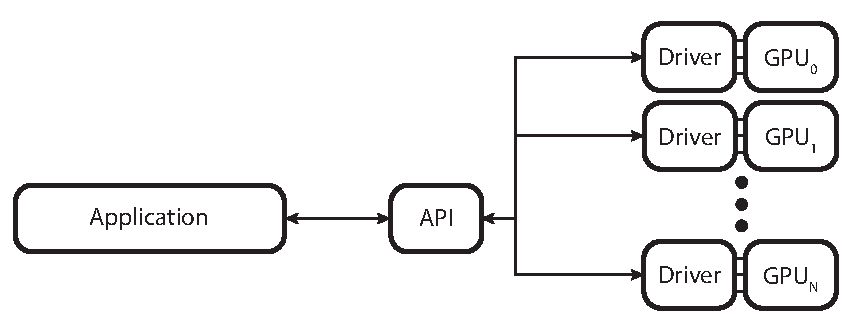
\includegraphics[width=\textwidth]{Main/Images/Application_API_Driver_Overview}
    \caption{Interaction between the application and the hardware via the API.}
    \label{fig:AppApiDriverOverview}
  \end{figure}

  Lorem ipsum dolor sit amet, consectetur adipisicing elit, sed do eiusmod
  tempor incididunt ut labore et dolore magna aliqua. Ut enim ad minim veniam,
  quis nostrud exercitation ullamco laboris nisi ut aliquip ex ea commodo
  consequat. Duis aute irure dolor in reprehenderit in voluptate velit esse
  cillum dolore eu fugiat nulla pariatur. Excepteur sint occaecat cupidatat non
  proident, sunt in culpa qui officia deserunt mollit anim id est laborum.

  Lorem ipsum dolor sit amet, consectetur adipisicing elit, sed do eiusmod
  tempor incididunt ut labore et dolore magna aliqua. Ut enim ad minim veniam,
  quis nostrud exercitation ullamco laboris nisi ut aliquip ex ea commodo
  consequat. Duis aute irure dolor in reprehenderit in voluptate velit esse
  cillum dolore eu fugiat nulla pariatur. Excepteur sint occaecat cupidatat non
  proident, sunt in culpa qui officia deserunt mollit anim id est laborum.

  \todo[inline]{Talk about different kinds of graphics \glspl{api} on different systems (D3D, OpenGL on desktop, maybe Metal for OSX, and special \glspl{api} on consoles.)}

  \section{Document Structure}
    Chapter~\ref{cha:Introduction} is the introduction to the topics discussed within this document.
    In chapter~\ref{cha:VulkanOverview}, an overview of the Vulkan graphics \gls{api} is given in terms of its components and features.
    Chapter~\ref{cha:EnvSetup} is a guide for setting up Vulkan for application development with a bias towards \gls{windows} platforms.
    Chapter~\ref{cha:RenderPipeline} sets up a simple rendering scenario and explains it step by step.
    And finally, chapter~\ref{cha:Conclusion} concludes this document and provides insight to thoughts of the author about the topics discussed.


  \section{High Level Graphics Workflow}
    \label{sec:GraphicsWorkflow}
    \todo[inline]
    {
      General overview of the stages several resources (vertices, textures, etc.) have to go through.

      Explain the fixed function stages.

      Mention that this is simplified!!! Mention there are more stages.
    }

    \todo[inline]{Change the text ``Vertex Data'' to ``Input Data'' in figure~\ref{fig:Rendering_Pipeline_Overview}.}
    \begin{figure}
      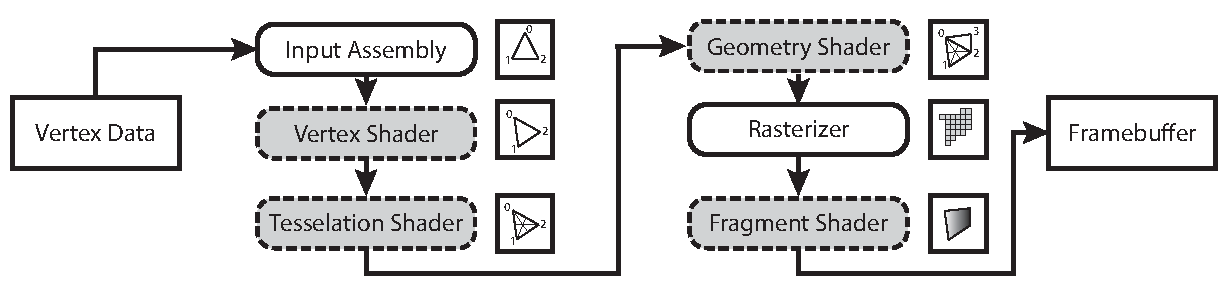
\includegraphics[width=\textwidth]{Main/Images/Rendering_Pipeline_Overview}
      \centering
      \caption{Fixed-function stages are depicted with solid, rounded outlines and shader stages with dashed outlines.}
      \label{fig:Rendering_Pipeline_Overview}
    \end{figure}

    Generally speaking, graphics hardware is built like a pipeline that is made up of several components called pipeline stages.
    Each of these stages is processing data that is provided by the \textit{host application}, before being passed on to the next stage in the pipeline.
    The pipeline stages can generally be categorized into fixed-function stages and shader stages.
    Fixed-function stages perform the same kind of operation on incoming data.
    Control over the operation is limited, but in many cases a fixed-function stage can be configured to some extent.
    Shader stages accept application-defined programs, called \textit{shaders}, that are run in order to process incoming data.
    \todo{...}Overview of the rendering pipeline on modern graphics hardware.
    The available shader stages are the vertex, tessellation, geometry, and fragment shader stages.

    % The input assembly, for example, is responsible for producing primitives from the input data for the vertex shader to consume.

    \begin{description}
      \item[Vertex Shader]
        Vertex shaders are invoked for individual vertices.
        This stage is typically used to transform vertices to different coordinate systems.

      \item[Tessellation Shader]
        Tessellation shaders are generally used to turn coarse geometry into smoother geometry by adding more detail.
        \todo[inline]{Used for water, e.g. or to create a mathematical ...}

      \item[Geometry Shader]
        Geometry shaders are used to generate new geometry from existing primitives.
        For example, the geometry shader may be used to turn a single vertex into a triangle.

      \item[Fragment Shader]
        Fragment shaders work on individual output pixels to determine values that are written to the framebuffer.
        In other words, this is the stage where the actual pixel colors are produced, optionally by sampling textures and applying lighting computations.
    \end{description}

    \todo[inline]{Is this enough for the \underline{high level} graphics workflow?}

  \section{Motivation for a new Graphics API}
    \todo[inline]{Hardware abstraction of old APIs based on old hardware design.
    \todo[inline]{Check for repetition.}
    Hardware design changed a lot (much more general purpose).
    Old APIs need to perform a lot of work to maintain the illusion of old hardware design.
    Special purpose hardware is largely replaced by general purpose memory and massively parallel processors for crunching data.}
    \todo[inline]{Different Formulation. Graphics hardware changes rapidly, etc...}
    Old graphics \glspl{api} were designed for old graphics hardware designs.
    However, hardware design has changed significantly over time.
    The model older graphics \glspl{api} are based on no longer reflects modern hardware design.
    In order to remain compatible, these \glspl{api} need to perform a mapping of their model to modern hardware design.
    This mapping may come at a significant cost in terms of performance.

    In practice, this often means that the hardware driver, implementing an old graphics \gls{api}, wastes a considerable amount of time that could be used by the host application to perform useful \todo{Use `operations' instead?}computations.
    For some applications, this \todo{``may be acceptible...'' is clearer}overhead caused by the driver is not very significant.
    Applications like these may not gain much by the new \glspl{api} other than lower power consumption due to reduced \gls{cpu} usage, which might be important on mobile platforms.

    Modern hardware design tends to be more suitable for general purpose computing compared to old hardware design.
    Older hardware consisted of many special purpose components that have largely been replaced by general purpose memory and programmable processing cores that perform work in a massively parallel manner.

    \todo[inline]{Main goal of modern APIs is to match modern hardware design. Enables drivers to work more directly with the hardware instead of perform a mapping between the abstract model and the actual hardware.}

    Modern graphics \glspl{api} match their abstraction closer to modern hardware design.
    This enables drivers to work more directly with the hardware and reduce the aforementioned cost of mapping the driver model to the actual hardware.
    This is arguably the main motivation for new graphics \glspl{api}.

    Another aspect of modern graphics \glspl{api} is the level of control that is given to the application.
    \todo{Don't be abstract: Mention directX, opengl, i.e. the established apis}Modern \glspl{api} tend to design their model much closer to the current hardware, exposing it a lot more than older \glspl{api} did.
    The fact that modern graphics hardware has become more general purpose is certainly a factor in this.
    Designing general purpose hardware only to be constrained by \glspl{api} that do not provide ways to leverage it would be a waste of resources.
    \todo{References??}Additionally, having more control of the hardware has been the desire of many developers in the past.
    On gaming consoles, for example, working closely with graphics hardware has been always possible\footnote{Except on \gls{ms} platforms where \gls{d3d} technology is used.}.
    A game ported from a console to a platform \todo{``such as''?}like the \gls{pc} would often run less optimal in comparison in terms of the most optimal use of available resources.

    Providing more control to the application also means that drivers have to do less guess-work to figure out what the application wants to do.
    This makes driver implementations simpler and easier to maintain, reducing the possibility for \glspl{bug}.
    \todo{Application developers have a better chance to optimize for different hardware.}
    \todo[inline]{The following sentence is not correct. Reformulate.}
    It also reduces the gap between different driver implementations, making applications work more consistently across hardware from different vendors.

    \todo[inline]{Secondary goal is to make drivers simpler at the cost of making applications more complicated. This is not necessarily bad because the application has control over how hardware is utilized. Drivers don't need to guess user intent as much anymore. Also, less complex driver means better maintainability and fewer bugs.}

    Multithreading is also a concern for modern graphics applications.
    With older graphics \glspl{api} it was usually much harder, if not impossible, to utilize multiple threads in terms of rendering.
    At the time these \glspl{api} were designed, applications were usually running only in a single thread.
    Modern graphics \glspl{api}, on the other hand, have been designed with multi-core processing in mind.

    \todo[inline]{Mention CPU overhead of GPU instructions, especially on mobile.}

    \todo[inline]{Talk about new APIs such as D3D12, Mantle, Metal, and also talk about consoles (no specs) that all adress these problems.}


  \section{The Vulkan Graphics and Compute API}
    \todo[inline]{What does it do. Where does it come from. What are people expecting from it. Cross-platform nature (in comparison maybe to PS4's libGNM made specifically for PS4 hardware).}

    \todo[inline]{Insert missing references.}
    The Vulkan \gls{api} was designed by the Khronos Group in collaboration with many industry representatives, including Valve Corporation, \gls{amd}, and \gls{nvidia}.
    Version 1.0 of the Vulkan specification was released on the 16th February in 2016.
    It was designed to provide low-level control to the developer when interacting with graphics and compute hardware.

    Vulkan was designed with a variety of goals in mind.

    \todo[inline]{Will this stay a list?}
    \begin{itemize}
      \item Cross-platform
      \item Keep driver complexity at a minimum
      \item Less driver-side \gls{cpu} overhead
      \item Allow developers a lot of control over the hardware
      \item Consistent API
    \end{itemize}

    There are many different kinds of hardware configurations today, ranging from high-end gaming systems to mobile platforms such as smartphones.
    Vulkan is designed to be used with all of these systems.
    There will be no special version of Vulkan dedicated to embedded systems as was the case with \gls{gles}.

    As a result of striving for less driver overhead, Vulkan also provides the possibility of reducing \gls{cpu} and \gls{gpu} power consumption.
    The driver implementation will have to make fewer guesses of what the host application is trying to do.
    It is up to the application developer to tell the Vulkan driver exactly what needs to be done.
    This way the driver only does as much work as it needs to function properly and less power will be consumed.
    Hardware vendors will also have an easier time providing robust drivers with less bugs due to reduced complexity.

    Another advantage of Vulkan, being a new API built without worrying about backwards compatability, is the chance of designing a new and consistent API so developers will have an easier time creating applications.
    For more information about the API structure and common patterns in Vulkan, see chapter~\ref{cha:VulkanOverview}.

    Version 1.0 of Vulkan was not entirely built in-house at Khronos Group but is in part based on components of AMD's Mantle API, which was donated to the Khronos Group.


    \subsection{Vulkan Competitors}
      \todo[inline]{OpenGL, Direct3D11, Direct3D12, libGNM (PS4), OpenCL}

      Other \glspl{api} exist that are direct competitors to Vulkan.

      \gls{opengl} is Vulkans predecessor and provides a higher level of abstraction from the hardware.
      It is a very successful API running on several different platforms with varying hardware configurations.
      Due to its level of abstraction, \gls{opengl} drivers are very complex and do a significant amount of work on the \gls{cpu} in order to match abstract commands to the hardware.

      Special flavors of \gls{opengl} exist, such as \gls{gles}, which is a subset of \gls{opengl} to enable hardware-accelerated graphics processing on embedded systems such as smartphones and tablets.

      The \gls{d3d} family of \glspl{api} is developed by Microsoft and only supports Microsoft platforms such as the Windows operating system or the Xbox gaming console.
      The most recent versions of \gls{d3d} are \acrlong{d3d11} and \acrlong{d3d12}.
      \acrlong{d3d11} provides a \todo{Compared to what? Make this un-ambiguous}higher level of abstraction from the hardware, similar to \gls{opengl}.
      It has been around since the release of Windows 7 in 2009.
      \acrlong{d3d12}, the latest revision of the \gls{d3d} specification released in 2015, is comparable to Vulkan in terms of of hardware abstraction.
      It provides much more control to the developer over the hardware.

      \todo[inline]{Mac OS X: Metal}

      \todo[inline]{Gaming console graphics libraries?}

      \todo[inline]{OpenCL as compute API}

  %!TEX root = ../Main.tex

\chapter{Vulkan API Overview/Workflow}
\label{cha:VulkanOverview}
  \todo[inline]
  {
    The Vulkan Graphics \acrfull{api} workflow, object creation, patterns (vkCreate/vkDestroy, vkAllocate/vkDeallocate), synchronization.

    Listing and short explanation of Vulkan components such as buffers, images, command buffers.

    Note that when talking about a ``device'', a logical device is meant. When referring to the actual hardware component the term ``physical device'' will be used.
  }

  \todo[inline]{Object/handle based with state-machines only for command buffers.}

  \lipsum

  \section{Workflow and Patterns}
  \label{sec:WorkflowAndPatterns}
    \lipsum

  \section{Layers and Extensions}
    \todo[inline]{Layers are instance-only, extensions are both on the isntance-level as well as the device-level.}

    Vulkan is designed to be extensible by thirdparty developers. The two mechanisms provided are called layers and extensions.

    A layer in Vulkan can be thought of as an observer to the API calls done by the developer. It does not add new types or functions the developer can use directly.\todo{Illustration of Vulkan with some layers between it and the user}\todo{Elaborate more to make it crystal clear. Make sure to mention no layers are needed.}

    The LunarG SDK, for example, comes with a set of layers to validate usage of the Vulkan API. This is extremely useful during development as it allows the developer to focus on their code rather than the perfect use of the Vulkan API. It should also be noted that bare Vulkan, without any validation layers enabled, does not do any error checking. When the developer passes an invalid combination of flags to some Vulkan function, it is undefined behavior and has to be corrected by the developer.

    Layers can only be created on the instance-level. Until version x.x.x.x \todo{Find out the exact version.}, the developer was able to create device-level layers, but these are deprecated in Vulkan version x.x.xx.x by now.

    \todo[inline]{Pull out neutral descriptions of layers/extensions and put the examples in their own paragraph.}

    As opposed to layers, extensions are able to provide new or add to existing functionality. The motivation for extensions is to keep the Vulkan core functionality small and provide specific functionality via such extensions. In fact, the Khronos Group itself provides built-in extensions for both common and platform specific functionality. An example of an extension that adds platform independent functionality is the \lstinline{VK_KHR_swapchain} extension. It adds several types and functions to create and interact with a swapchain. The concept of a swapchain itself is independent of the platform but it requires the help of platform specific functionality in order to work. On Windows platforms, for example, the developer needs to enable the \lstinline{VK_KHR_win32_surface} extension in order link a swapchain to a Win32 window. From a developer's perspective, they do not have to care about distinguish between platforms when creating a swapchain but they do have to when creating and connecting the swapchain to a surface.

    Extensions can be enabled on both instance-level and device-level. Instance-level extensions provide functionality that is generally independent of the hardware.

    An example for an instance-level extension is \lstinline{VK_EXT_debug_report}. It enables the developer to provide a callback function that is used by Vulkan layers or extensions to communicate with the developer. If validation layers are enabled, this is how they would tell the developer about any validation concerns or violations. An example for a device-level extension is the aforementioned \lstinline{VK_KHR_swapchain} extension. Not all physical devices have to be capable of rendering graphics images. In the end it is up the extension author on which level they provide their extension.

  \section{Memory Management}
    \todo[inline]{Allocate memory separately and then binding it to resources. Decoupled on purpose for custom management.}

    Memory management is an important topic in Vulkan.

    \lipsum

  \section{Shader Language: SPIR-V}
    \todo[inline]{\acrfull{spirv}}

    \lipsum

  \section{Synchronisation Primitives}
    \todo[inline]{Describe what Vulkan offers and discuss the individual use-cases as well as their performance impact.}

    \lipsum

  \section{Interaction with the Operating System}
    \todo[inline]{Windowing system, specific Vulkan extensions per OS.}

    \lipsum

  %!TEX root = ../Main.tex

\chapter{Vulkan Development Environment}
\label{cha:EnvSetup}
  \todo[inline]
  {
    High level goals of this chapter:

    -- Generating `vulkan.h'

    -- LunarG SDK

    -- Installing layers

    -- Present most important layers / extensions
  }
  \todo[inline]
  {
    Buzzwords: Tools, development environment, Vulkan in practice
  }

  \tbd

  %!TEX root = ../Main.tex

\chapter{Rendering Pipeline}
\label{cha:RenderPipeline}
  \todo[inline]
  {
    Possible titles:

    -- Rendering Workflow

    -- Applying the Rendering Pipeline

    -- Rendering in Vulkan

    -- Rendering Commands and Resource Handling/Management
  }

  \todo[inline]{Pipeline creation? caching?}
  \todo[inline]{Command buffer building. (CBs can be viewed as functions).}
  \todo[inline]{Communication with the GPU}
  \todo[inline]{Image tiling and layout}
  \todo[inline]{Resource transformations.}
  \todo[inline]{Command buffer submission. Mention out-of-order execution. Analogous to CPU instruction dispatch.}
  \todo[inline]{Command buffers can be built once and submitted multiple times. Better performance because no upload (and other things).}
  \todo[inline]{"Setup command buffers", "Draw command buffers", "pre/post-draw command buffers"}
  \todo[inline]{Binding of resource to memory: bind a dummy for as long as the resource loads.}
  \todo[inline]{Diagram for overview of the "pipeline" to give an idea of the whole thing.}

  This chapter describes a set of basic steps to get an image on the screen.
  It assumes a swapchain is set up and ready to be used using the swapchain extension as described in section~\ref{sec:WorkflowAndPatterns}.

  % Command buffers are not unlike procedures where every instruction within that procude is dynamically recorded at runtime.
  % Just like procedures on the \gls{cpu}, command buffers translate to machine instructions on the \gls{gpu}.
  % When a command buffer is submitted, commands within that command buffer may be executed out-of-order, i.e.
  % in another order than they were recorded, if the \gls{driver} or the \gls{gpu} decide to be more efficient in some way.

  % There are two kinds of command buffers: primary command buffers and secondary command buffers.
  % Primary command buffers may be directly submitted to a device queue.
  % Secondary command buffers, on the other hand, must be executed as part of a primary command buffer.
  % The Vulkan command \lstinline{vkCmdExecuteCommands} may be used for this.
  % \todo{Find out more about secondary command buffers!}Secondary command buffers are basically like macros.
  % Secondary command buffers inherit some state form the calling primary command buffer.

  This section will define the framework for the rest of the chapter.
  All examined use-cases of the Vulkan API are moving within this framework.

  \todo[inline]{Vulkan provides many ways to render. In this chapter, one of many ways is explored from beginning to end to show stuff.}

  \todo[inline]{Free moving camera.}
  \todo[inline]{Objects with fixed geometry.}
  \todo[inline]{No complex shading - flat lighting.}
  The graphics scene is kept very simple.
  It only contians objects with fixed geometry.
  The geometry itself may be arbitrarily complex because it has no impact on the usage of the \gls{api}.
  Shaders are also kept simple because this area is not important enough for what is examined in this chapter.

  The shaders used in this chapter are kept very simple.
  Other aspects of Vulkan are more important for this chapter.
  Each object is limited to a single sampled image to be used as a texture.
  As for lighting objects, simple flat shading is performed.
  A vertex consists of the following elements.
  \begin{itemize}
    \item Three \lstinline{float} values representing the position of the vertex in \gls{3d} space.
    \item Two \lstinline{float} values representing the coordinates of the vertex in texture space.
  \end{itemize}

  \todo[inline]{Bring the following into better form.}
  Restrictions:
  \begin{itemize}
    \item Rendering to single window / surface
    \item Forward renderer / single render target
    \item Simple shaders only
    \item Static geometry (no morphing)
    \item Freely moving camera
    \item ...
  \end{itemize}

  \begin{figure}
    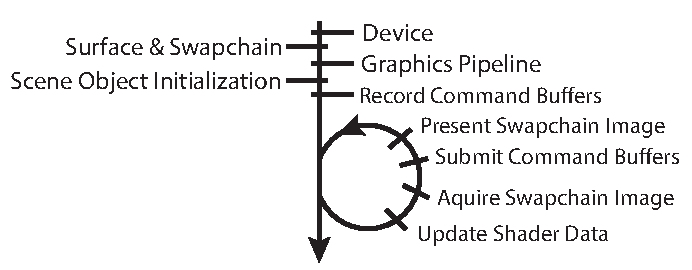
\includegraphics{Main/Images/RenderSetupAndLoopSimple}
    \centering
    \caption{Overview of the setup and execution for a simple forward-render in Vulkan.}
    \label{fig:RenderSetupAndLoopSimple}
  \end{figure}

  \section{Framework}
    \label{sec:Framework}
    \todo[inline]{Explain why this framework is needed. Vulkan offers many possibilities and each application by do things differently.}
    \todo[inline]{Forward renderer.}
    A simple forward renderer is assumed.
    \todo[inline]{Scene with discrete number of objects.}
    The rendered scene will contain a discrete number of objects.
    \todo[inline]{Each object has fixed geometry and a single texture.}
    Each object has fixed geometry and is assigned a single texture.
    \todo[inline]{Single camera that is movable.}
    A camera is used to observe the scene.
    This camera is also movable, e.g. by user-input.
    \todo[inline]{Realtime rendering? Might not be relevant.}
    \todo[inline]{Simple shaders, contents not relevant.}
    Simple shaders are used to render each object of the scene.
    The exact contents of these shaders is not relevant.
    The layout of these shaders is discussed at a later point.

  % \section{Requirements}
  %   Some requirements arise from the framework defined in section~\ref{sec:Framework} which are discussed in this section.
  %   A central requirement is the render target.
  %   Since the ultimate result of a rendering pass is to produce a presentable image, the render target will be an image of the swapchain.
  %   Thus, a swapchain setup as discussed in section~\ref{sec:Pipelines} is required.
  %   In order for each object to be sorted properly during rendering, a depth buffer needs to be set up for the rendering pipeline.

  \section{Setup}
  \label{sec:RenderingSetup}
    \todo[inline]{Before it's possible to render, certain things need to be set up.}
    Before it is possible to start rendering an image, proper Vulkan facilities need to be set up.
    These are discussed in section.
    The setup here adheres to the framework defined in section~\ref{sec:Framework}.

    \subsection{Creating a Proper Device}
      The Vulkan device that is to be used for rendering needs to support both the swapchain extension and queues with graphics and present capabilities.

      In order for a rendered image to be presented to a window, the swapchain extension\footnote{Full name: \lstinline{VK_KHR_swapchain}} needs to be activated.
      This can be done when creating the device.
      Without this extension, no swapchain can be created for this device, which is necessary to present a rendered image in Vulkan.
      Note, however, that the swapchain is not created at this point.
      This has to be done explicitly by the application and is explained later.

      In Vulkan, rendering commands are submitted to a device queue.
      For the purposes of this chapter, queues with two specific capabilities are required.
      These capabilities are called the \textit{graphics capability} and the \textit{present capability}.
      \todo{Is it important \textbf{how} to get the info about the capabilities?}The first specifies whether the queue supports graphics commands such as \lstinline{vkCmdDraw}.
      The second capability specifies whether \lstinline{vkQueuePresentKHR} is supported on that queue.
      Without both of these capabilities, rendering and presenting an image is not possible.
      \todo{Rephrase}A queue might support both of these capabilities but it is also possible that two separate queues are used for graphics and presenting, respectively.
      Once proper queues have been chosen, a logical device can be created.
      This logical device will be used for all subsequent Vulkan operations.
      The queues that were created along with the logical device will be used to submit rendering commands to the \gls{gpu} and to trigger the presentation engine.

    \subsection{Creating a Surface and a Swapchain}
      \todo[inline]{Setup of OS specific surface and swapchain.}
      Now that a device with the enabled swapchain extension is in place, a swapchain can actually be created.
      Creating a swapchain requires what is called a Vulkan \textit{surface} to be created first.
      This surface is operating specific and represents the connection to the actual window.
      It is also the target of the presentation engine, i.e. that surface is used to present a rendered image.

      \todo[inline]{Number, format, extent, colorspace of swapchain images.}
      \todo[inline]{Present modes / VSync.}
      A swapchain consists of multiple images.
      These images are managed by the presentation engine.
      The application may require the swapchain to create a certain number of images constrained to a range defined by the surface.

      \todo[inline]{Move this either to chapter 2 or 3. In this chapter, we mainly care about setting up the swapchain for the framework defined above.}
      The reason why an application may care about the number of swapchain images is rather straight-forward.
      A swapchain image passes some stages until is presented eventually.
      Initially the image is free and can be acquired by the application.
      Once an application acquires the image it is considered to be in use by the application and no longer free.
      At some point, the application hands back the image to the presentation engine, requesting that image to be presented.
      \todo{Explain more presentation modes?}In the \gls{fifo} presentation mode, the image will be put into a queue to be processed by the presentation engine at a convenient time.
      Once that time has come, the image will actually be presented on the surface.
      While an image is either currently presented or still pending presentation in the queue, it cannot be acquired by the application for rendering.
      When there is no free swapchain image, and the application tries to acquire one, the application will be stalled until a swapchain image is available.
      Depending on the chosen presentation mode, the number of swapchain images can be tuned to find the balance that works best for the application.
      Using too many swapchain images wastes memory but not having enough images may stall the application.

      \todo[inline]{Transform mode? Not really relevant for this chapter, right?}
      \todo[inline]{Usage? Swapchain images can always be used as color attachment.}
      Swapchain images will be used exclusively as color attachments for the framebuffer.

    \subsection{Creating a Graphics Pipeline}
      \todo[inline]{Create depth buffer}
      A depth buffer also needs to be created and used within the render pass in order for the objects to be rendered correctly according to how they are ordered.

      \todo[inline]{Create framebuffer for each swapchain image, a render pass, and graphics pipeline. }
      \tbd

    \subsection{Creating Scene Objects}
      \todo[inline]{Create renderable objects. Needs sampled image, geometry. Mention push constants.}
      \tbd

  \section{Command Buffer Recording}
  \label{sec:BuildCommandBuffers}
    \todo[inline]{Mention that this is done on a single thread.}
    \todo[inline]{Mention that this may be done once or multiple times, depending on use of push constants and other things.}
    \todo[inline]{Build command buffers that will never change. Depend on whether push constants are used or not.}
    \todo[inline]{Image layout transition with barriers.}

  \section{Rendering Loop}
  \label{sec:RenderLoop}
    \todo[inline]{Rather simple because of pre-recording command buffers.}
    \todo[inline]{Update uniform buffers.}
    \todo[inline]{Possibly explain push constants.}
    \todo[inline]{Acquire swapchain image.}
    \todo[inline]{Submit command buffers.}
    \todo[inline]{Present swapchain image.}
    \todo[inline]{Sync for submission and presenting (render semaphore, present semaphore) so swapchain image isn't used for rendering while presenting and vice versa. Also image layout transition happens with commands, meaning sync is necessary!}
    \tbd

  \section{Window Resizing}
    \todo[inline]{Should I actually add this section? (Only if there's enough time.)}
    \tbd

  \section{Multi-threaded Rendering}
  \label{sec:MultithreadedRendering}
    \todo[inline]{Introduction to this chapter. Motivation. Additional complexity. Applications must be sure they gain anything from using multi-threading.}
    As mentioned in chapter~\ref{cha:VulkanOverview}, the \gls{driver} has only limited support for multi-threaded access.
    However, this does not mean that multi-threading on the \gls{cpu} has not been taken into account when Vulkan was designed.
    There are actually several ways of utilizing multiple threads for rendering with Vulkan.
    Creating resources and recording command buffers from multiple threads are explored in the following subsections.

    \subsection{Multi-threaded Command Buffer Recording}
      A naive approach to utilize multi-threading is to create several command buffers and assign them to multiple threads.
      These threads would then record commands to their assigned command buffers and submit them to a device queue.
      Unfortunately, there are some problems with this approach.
      According to sections~5.3~and~5.4 of the Vulkan specification\cite{vkspec}, the host application is responsible for synchronizing interactions with command buffers and submitting them to device queues.

      % Problem with command buffers and multi-threaded access.
      Command buffer access is not thread-safe.
      This is because memory used by command buffers is managed by the parent command pool.
      The actual algorithms used for managing memory are left to the \gls{driver}.
      % Done for implementations to be more memory efficient.
      This allows command pools efficient handling of memory operations performed by multiple command buffers, e.g. by allocating more memory than is currently needed and reassigning it as more is requested.
      % Command buffers work on memory managed by parent command pool.
      Because command pools are free to manage memory as they see fit, any operation on a command buffer may trigger side-effects that affect other command buffers created from the same pool.
      This fact alone makes command buffers unsuitable to be shared across multiple threads without synchronization.

      % Command pools do not depend on anything else.
      Command pools, on the other hand, are independent objects.
      The memory they manage is only used for command buffers they created.
      Whenever available memory is no longer sufficient, new memory from the host is requested, optionally using a application-supplied allocator.
      This allocator needs to synchronize low-level allocations, like the C standard library function \lstinline{malloc} already does.
      % Thus solution is to assign each thread its own command pool.
      Synchronization of low-level memory allocation is certainly not as costly as synchronizing each command buffer access.
      Typically, those low-level memory allocations do not happen very often.
      It is likely that command pool implementations strive for minimal host allocations.

      Command pools effectively do not need to be manually synchronized across multiple threads if they are not shared between them.
      In addition, command buffers created from such command pools inherit the same properties.
      Thus, it is more suitable to assign one or more command pools per thread.
      % Threads then allocate and record into as many command buffers as needed.
      Each thread is then free to allocate and record into as many command buffers as needed without having to conduct fine-grained synchronization.

      % Let main thread submit command buffers by sharing a datastructure with synchronized access.
      In order for command buffers allocated on other threads to be submitted to the device queue, the main thread may provide a shared datastructure that is capable of containing command buffer objects.
      Access to this shared container would be synchronized using traditional synchronization methods.
      % Turns the initial problem into well-understood producer-consumer problem\cite{EWD:EWD329}.
      % Solves the inital queue submission problem.
      This effectively creates the well-understood producer-consumer scenario\cite{EWD:EWD329} and solves the initial queue submission problem.

      \todo[inline]{Prev paragraph is just a suggestion. May be better to do differently. Depends on application.}

      \subsubsection{Command Buffer Management Considerations}
        % ... There is another problem with the system mentioned above.
        % ... It is also recommended to assign more than one command pool to an individual thread.
        % ... While a command buffer is being processed, i.e. once it has been submitted but has not finished execution yet, the command buffer should not be modified.
        % ... The reason why multiple pools should be used instead of simply creating new command buffers from the same pool is because of the underlying memory model.

        % ... In the previously described scenario, each thread has exactly one command pool that is used to create multiple command buffers from.
        % ... Commands are recorded to these command buffers and are submitted in batches to the device for execution.
        % ... Vulkan specifies some restrictions on what may be done with command buffers that are pending execution.
        % ... For example, the application should not free a command buffer that is pending execution.

        % Command buffers need to be kept alive while pending execution.
        Vulkan prohibits modifying submitted command buffers that are pending execution on the device.
        This includes freeing these command buffers, i.e. the application is responsible for keeping them alive as long as they are pending execution.
        In practice, this effectively means command buffers submitted in batches may only be modified or reused once the entire submission has finished execution because it is hard to predict when individual commands are processed if more than one command buffer is submitted.
        Out-of-order execution is one reason for this unpredictability.
        The simplest way to solve this problem is to just use new command buffers for every new batch submission.
        This poses some management overhead since individual command buffers need to be associated to these batches in some way in order to be freed or reused.
        Vulkan does not do this automatically.
        Otherwise, if command buffers are never freed, the application ends up allocating a lot more than necessary, effectively leaking memory.

        % Command pools better than just using command buffers because of decoupled underlying memory and clean separation of concern.
        A better way might be to use command pools for this purpose.
        Managing command buffers is already what they do and it also offers a clean separation of concerns between the different batches of command buffers.
        In other words, using command pools to allocate command buffers that are submitted together provides a way to manage these command buffers using standard methods.
        Vulkan allows command pools to be reset, effectively resetting all command buffers spawned from them, respectively.
        This means that command pools may be reused after their associated batch of submitted command buffers has finished execution.
        When resetting a command pool, the host application is free to choose whether memory allocated by that command pool should be released or not.
        If a command pool is going to be reused, and the memory is not released, this command pool can directly start producing command buffers without causing additional allocation overhead.
        This provides a clean way for managing command buffer lifetimes without the need to use anything but the Vulkan \gls{api} itself.

        \todo{Describe what they did differently?}Similar approaches have been described by industry experts such as Marius Bjørge\cite{bjorge:multithreadingvulkan} in his blog post about multi-threading in Vulkan as well as Mathias Schott\cite{mschott:vulkan_multi_threading} in his talk entitled "Vulkan multi-threading".

        Care must be taken, however, in cases where the amount of memory required by a command buffer is not steady during its lifetime.
        For example, when transitioning from a large \gls{3d} scene, with many objects to render, to a small scene with less draw calls to perform, the memory requirements of each command buffer may be lowered considerably for the new scene.
        In cases like this, it might make sense to reset all relevant command buffers, freeing their associated memory.
        Switching from a small scene to larger one is not a problem, of course, because the command buffer will simply allocate enough memory for the new scene.


    \subsection{Multi-threaded Resource Creation}
      Vulkan applications need to create resources such as images and shaders.
      Loading and creating these resources may take a considerable amount of time, depending on the data in question.
      Images, for example, can be quite large.
      They may also have to be transformed in some way which also consumes computation time.
      Shaders need to be compiled (by the \gls{driver}) and bound to a Vulkan pipeline.
      Many of these time consuming operations work more or less independently from the rest of the system, depending on the specific operation.
      This makes them interesting candidates for execution on multiple threads.
      However, the use of multi-threaded resource creation introduces additional complexity to the system.

      First of all, an application has to decide how many threads are actually needed for resource creation.
      It is possible that only one dedicated resource creation thread is sufficient for many applications.
      The actual number of resource creation threads depends on the application.

      All resource creation threads need device memory in one way or another.
      There are basically two ways of accomplishing this without race conditions.
      The first way is to preallocate the memory that is available for each thread.
      This method does not require synchronization between threads because each is assigned a memory region that is not overlapping memory from other threads.
      The second way is to assign a memory allocator to each thread that internally synchronizes the calls.
      This method does not require the main thread to know the size of the resources each thread creates but memory allocations need to be synchronized.
      Again, the method of choice depends on the application.

  % %!TEX root = ../Main.tex

\chapter{Prototype}
\label{cha:Prototype}
  \todo[inline]
  {
    High level goals of this chapter:

    -- Show some practical parts of using Vulkan.

    -- Present implementation of parts previously discussed concepts.

    -- Command buffer recording code.

    -- SPIR-V converter.

    -- Omit host-side multithreading.
  }

  \tbd

  %!TEX root = ../Main.tex

\chapter{Conclusion}
\label{cha:Conclusion}
  \todo[inline]
  {
    API quality. Explain and discuss why the API is called `modern', `highly efficient', and `explicit'.
  }

  \tbd



  \newpage
  \pagenumbering{Roman}


  %
  % Bibliography
  %
  \newpage
  % Print all bibliography entries.
  % \nocite{*}
  \printbibliography[heading=bibintoc,title=Bibliography]


  %
  % Glossary
  %
  \printnoidxglossaries

  %
  % Appendix
  %
  %!TEX root = ../Main.tex

\appendix

%
% List of Figures
%
% \chapter{List of Figures}
% \label{cha:ListOfFigures}
% \cleardoublepage
% \phantomsection
% \addcontentsline{toc}{section}{\listfigurename}
% \begingroup
%   \let\clearpage\relax
%   \listoffigures
% \endgroup
\listoffigures

%
% List of Tables
%
% \chapter{List of Tables}
% \label{cha:ListOfTables}
% \cleardoublepage
% \phantomsection
% \addcontentsline{toc}{section}{\listtablename}
% \begingroup
%   \let\clearpage\relax
%   \listoftables
% \endgroup
\listoftables


\end{document}
